\section{Trasformazione del modello E/R}
Riferendoci al modello raffigurato in \ref{fig:er} possiamo cominciare
a discutera della semplificazione e della specializzazione del
modello. Partendo dal modello \ref{fig:er} possiamo vedere come gli attributi:
\begin{description}
\item[descrizione] dell'entità \textbf{Intervento}
\item[posizione] dell'entità \textbf{Sensore}
\end{description}
siano composti. Di conseguenza è possibili trasformarli nel seguente modo:
\begin{center}
  descrizione $\rightarrow$ sostituzione,riparazione, calibrazione
\end{center}
e
\begin{center}
  posizione $\rightarrow$ latitudine, longitudine, altitudine
\end{center}

Di conseguenza il modello diventa
\begin{figure}[ht]
  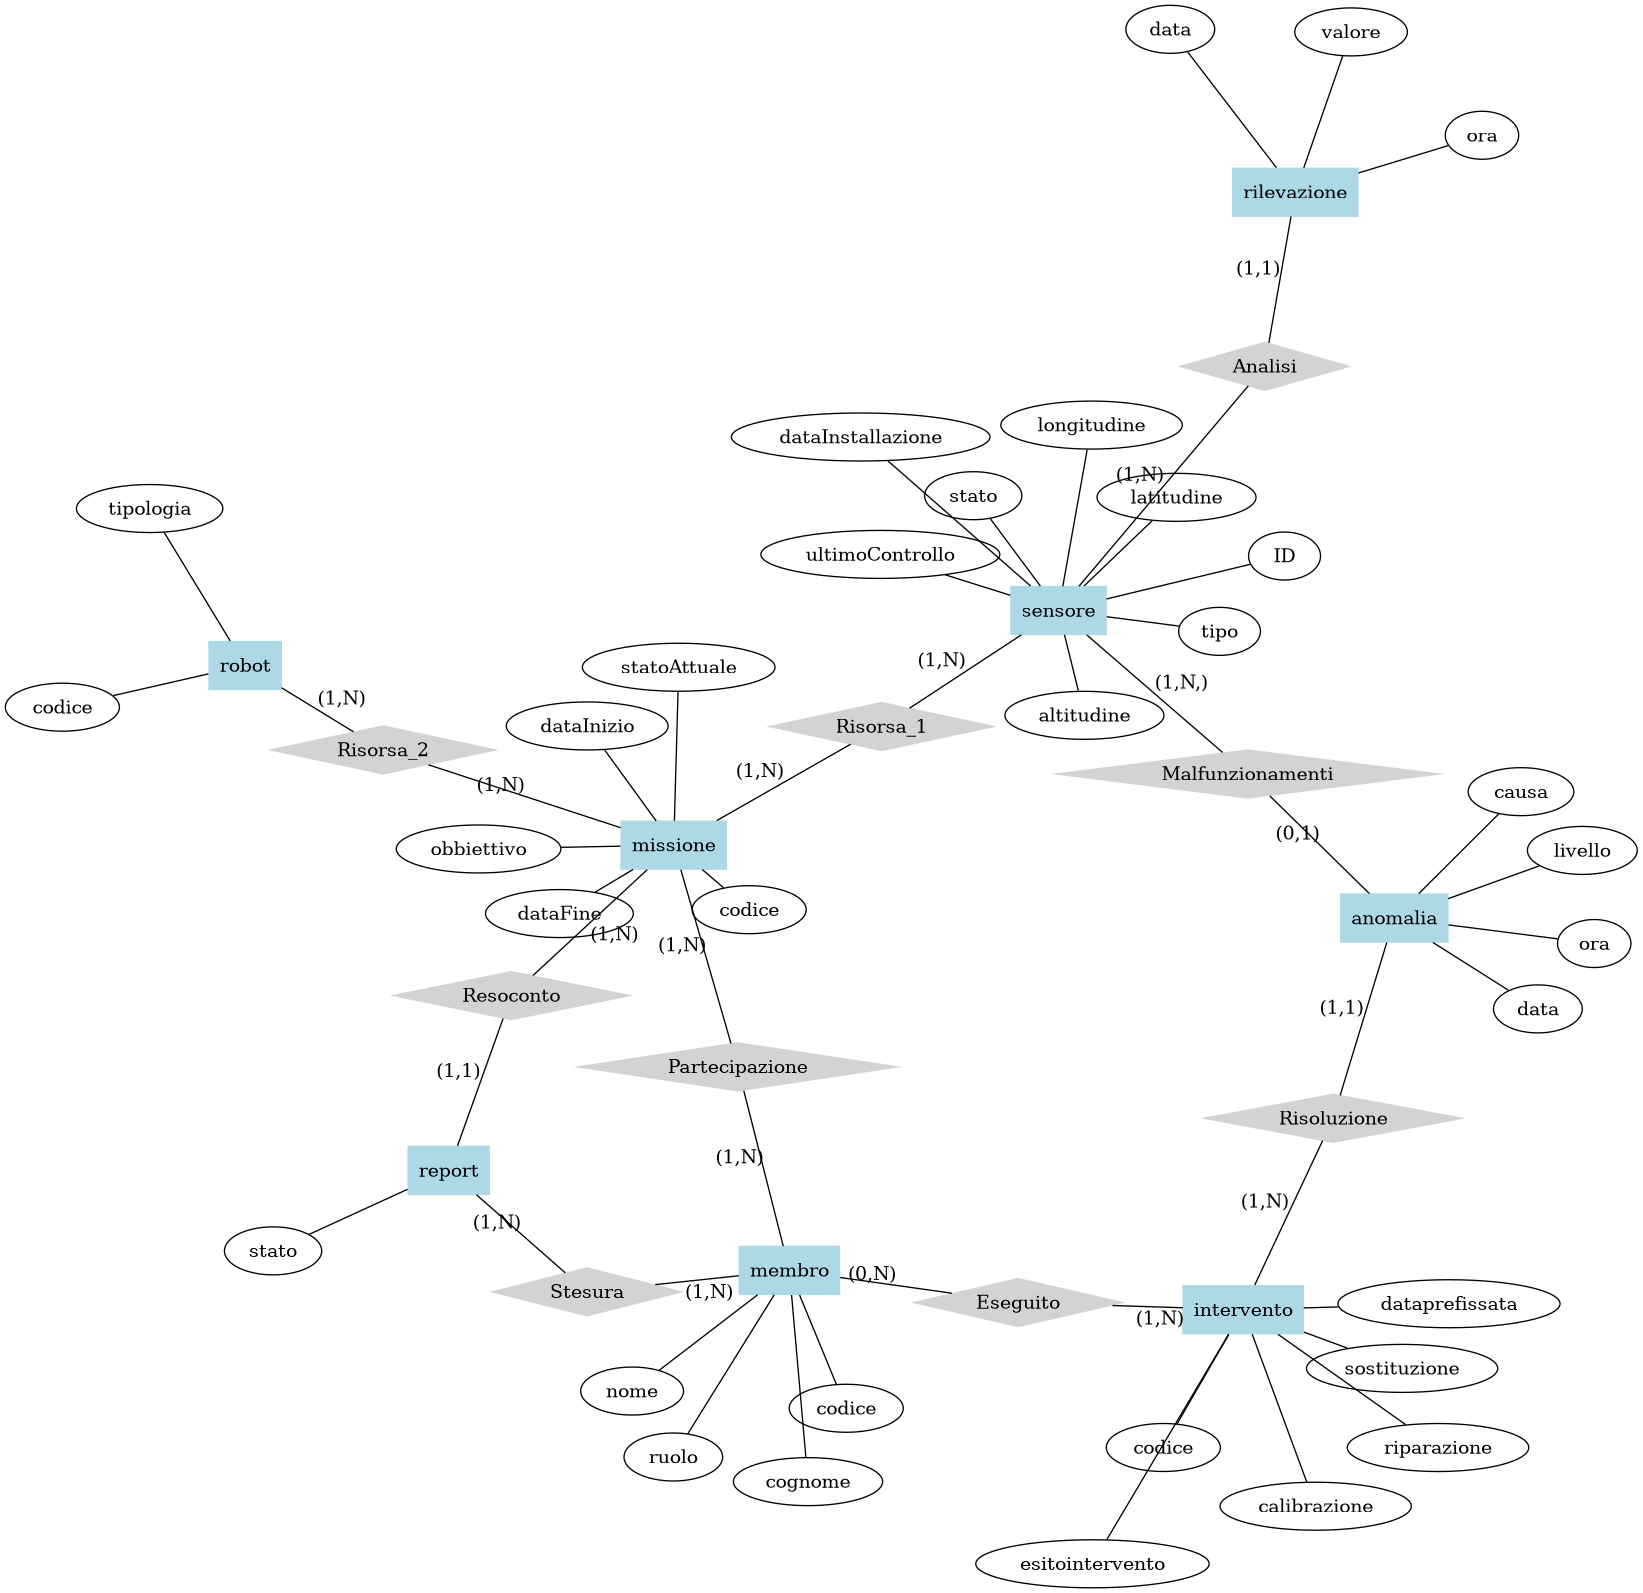
\includegraphics[width=\linewidth]{images/er-finale.png}
  \caption{Modello ER finale per \texttt{ASTRADM}}
  \label{fig:er-finale}
\end{figure}
 	
%%% Local Variables:
%%% mode: LaTeX
%%% TeX-master: "Tesina"
%%% End:
